%====================================================================
%                 B E S S E L   F U N C T I O N S
%====================================================================

Bessel functions are named after Friedrich Wilhelm Bessel as he was the first to generalise them. The first use of Bessel functions is generally acredited to Daniel Bessel, who used the function of zero order in his work as an astronomer. There are three problems that encouraged the development of this theory in the beginning. These are: the motion of a body in an elliptic Kepler orbit, oscillations of a chain suspended at one end, and heat conductivity in a solid cylinder. Now a days, applications are found in all areas of mathematical physics which use the theory of wave motion.

\section{Bessel functions of the first kind}
Bessel functions are solutions to the Bessel differential equation.
%
%-----------------defn: bessel differential equation------------------
%
\begin{defn}The Bessel differential equation of order $\nu$ and argument $z$
  \begin{equation}\label{eq:bessel_differential}
      z^2 \frac{d^2 U}{dz^2} + z\frac{dU}{dz} + (z^2 - \nu^2)U = 0
  \end{equation}
for $\nu, z \in \bb{C}$.
\end{defn}\par
%
Throughout this project we will only be concerned with Bessel functions of integer order only, so we replace $\nu \in \bb{C}$ with $n \in \bb{Z}$. This will become clear in the next chapter.
%------------------------defn: bessel function------------------------
%
\begin{defn}\label{defn:bessel_func}
Bessel functions are defined as follows,
  \begin{align*}
      J_n(z) = \sum^\infty_{m=0} \frac{
      (-1)^m (z/2)^{2m+n} }{
      m! \Gamma(n+m) }
  \end{align*}
where $\Gamma(n)$ is the extension of the factorial $n!$ for $n \in \bb{Z}^{\geq 0}$ to the complex plane. We cannot simply use $n!$ because Bessel functions are defined for $n \in \bb{Z}^{< 0}$ as well.
\end{defn}
%
%------------propn: bessel function solves bessel equation------------
%
\begin{propn} Bessel functions of integer order solve the Bessel differential equation.
\end{propn}
\begin{proof} The proof in \parencite{korenev02bessel_func} is conceptually similar to this but is given in much less detail.\par
  %
  We begin by proposing a solution to the Bessel differential equation \eqref{eq:bessel_differential} in the form of a power series expansion
    \begin{equation*}
      U(z) = \sum_{m=0}^\infty c_m z^{m + \zeta}
    \end{equation*}
  and we assume that $c_0 \neq 0$. This will become relevant later. This allows us to find expressions for the first and second derivatives,
    \begin{align*}
      U'(z) &= \sum_{m=0}^\infty c_m (m+\zeta) z^{m+\zeta-1}, \\
      U''(z) &= \sum_{m=0}^\infty c_m (m+\zeta)(m+\zeta-1) z^{m+\zeta-2},
    \end{align*}
  which can be substituted into \eqref{eq:bessel_differential},
    \begin{multline}\label{eq:bessel_proof_summation}
      z^2 \left\{ \sum_{m=0}^\infty c_m (m+\zeta)(m+\zeta-1) z^{m+\zeta-2}\right\} \\
        + z \left\{ \sum_{m=0}^\infty c_m (m+\zeta) z^{m+\zeta-1} \right\}
          + (z^2 - n^2) \left\{ \sum_{m=0}^\infty c_m z^{m + \zeta} \right\} = 0.
    \end{multline}
  Consider the expansion of the first two terms of these sums,
    \begin{multline*}
      c_0(\zeta)(\zeta-1)z^{\zeta} + c_1(\zeta+1)(\zeta)z^{\zeta+1} + \sum_{m=2}^\infty c_m (m+\zeta)(m+\zeta-1) z^{m+\zeta} \\
      + c_0(\zeta)z^{\zeta} + c_1(\zeta+1)(\zeta)z^{\zeta+1} + \sum_{m=2}^\infty c_m (m+\zeta) z^{m+\zeta} \\
      - n^2 c_0 z^{\zeta} - n^2 c_1 z^{\zeta+1} -n^2 \sum_{m=2}^\infty c_m z^{m + \zeta} + \sum_{m=0}^\infty c_m z^{m + \zeta+2} =0.
    \end{multline*}
  Collecting terms we get
    \begin{multline*}
      z^{\zeta} \{ c_0(\zeta)(\zeta-1) +  c_0(\zeta) - n^2 c_0 \}
      + z^{\zeta+1} \{  c_1(\zeta+1)(\zeta) + c_1(\zeta+1)(\zeta) - n^2 c_1\} \\
      + \sum_{m=2}^\infty \left\{ c_m (m+\zeta)(m+\zeta-1) z^{m+\zeta} + c_m (m+\zeta) z^{m+\zeta} - n^2 c_m z^{m + \zeta} \right\} \\
      + \sum_{m=0}^\infty c_m z^{m + \zeta+2} =0.
    \end{multline*}
  Consider a change of variable to a dummy variable $m'$ for the last term: $m'=m+2$. Then we have $m=0 \Rightarrow m'=2$, $m\rightarrow \infty \Rightarrow m' \rightarrow \infty$ , and $m'= m-2$. So we can rewrite the last term as a sum from $m=2$,
    \begin{equation}
      \sum_{m=2}^\infty c_{(m-2)} z^{m + \zeta} =0.
    \end{equation}
  Hence we are left with the following expression
    \begin{equation}
      z^{\zeta} c_0\{ \zeta^2 - n^2\} + z^{\zeta+1} c_1 \{ (\zeta+1)^2 -n^2\}
      + \sum_{m=2}^\infty \{ c_m [(m+\zeta)^2 -n^2] + c_{m-2} \}z^{m + \zeta} =0.
    \end{equation}
  This must be valid for all $z \in \bb{C}$, so all the coefficients of $z^{\zeta +m}$ must be equal to zero.
    \begin{gather}
      c_0\{ \zeta^2 - n^2\} = 0,\label{proof:bessel_c0} \\
      c_1 \{ (\zeta+1)^2 -n^2\} = 0 \label{proof:bessel_c1}\text{ and}\\
      c_m [(m+\zeta)^2 -n^2] + c_{m-2} = 0 \text{ for } m \in \bb{Z}^{\geq 2} \label{proof:bessel_cm}
    \end{gather}
  First consider \eqref{proof:bessel_c0}. We assumed at the start that $c_0\neq0$, so we must have that
      \begin{equation}
        \zeta = \pm n.
      \end{equation}
  Additionally, from \eqref{proof:bessel_cm} we can see that there is a recursive relationship between all the coefficients $c_i$. Namely,
    \begin{align}
      c_m &= - \frac{c_{m-2}}{(m+\zeta^2)-n^2} = - \frac{c_{m-2}}{(m^2 +2m\zeta + \zeta^2 -n^2} \\
      &= - \frac{c_{m-2}}{m(m +2\zeta)} \text{ since } \zeta^2 = n^2,
    \end{align}
  and we can find the next terms in the sequence of coefficients for even $m$:
    \begin{align*}
      c_2 &= - \frac{c_0}{4(1+\zeta)}, \\
      c_4 &= - \frac{c_2}{8(2+\zeta)} = \frac{c_0}{4 \times 8 \times (1+\zeta) (2+\zeta)}, \\
      c_6 &= - \frac{c_3}{12(3+\zeta)} = - \frac{c_0}{4 \times 8 \times 12 \times (1+\zeta) (2+\zeta)(3+\zeta)}, ...
    \end{align*}
  Setting $\zeta = n$ we get the first partial solution for \eqref{eq:bessel_differential}
    \begin{align*}
      U_1(z) = c_0z^n \left\{
        1 - \frac{z^2}{4(1+n)} + \frac{z^4}{2!4^2(1+n) (2+n)} - \frac{z^6}{3!4^3(1+n)(2+n)(3+n)} + ...
        \right\},
    \end{align*}
  and setting $\zeta = -n$ we get a second partial solution
    \begin{align*}
      U_2(z) = c'_0z^{-n} \left\{
        1 - \frac{z^2}{4(1-n)} + \frac{z^4}{2!4^2(1-n) (2-n)} - \frac{z^6}{3!4^3(1-n)(2-n)(3-n)} + ...
        \right\}.
    \end{align*}
  For simplicity, the constants $c_0$ and $c'_0$ are set the following values.
  \begin{multicols}{2}
    \noindent
    \begin{align*}
      c_0 = \frac{1}{2^n \Gamma(1+n)}
    \end{align*}
    \begin{align*}
      c'_0 = \frac{1}{2^{-n} \Gamma(1-n)}
    \end{align*}
  \end{multicols}\par
  %
  Consider the first solution. Note that for $n \in \bb{Z}^{\geq0}$, $\Gamma (n+1) =n!$
  \begin{align*}
    U_1(z) &= \frac{1}{2^n n!} z^n \left\{
        1 - \frac{z^2}{2^2(1+n)} + \frac{z^4}{2!2^4(1+n) (2+n)} - \frac{z^6}{3!2^6(1+n)(2+n)(3+n)} + ...
        \right\},\\
      &= z^n \left\{
        1 - \frac{z^2}{2^{2+n} n!(1+n)} + \frac{z^4}{2!n! 2^{4+n} (1+n) (2+n)} - \frac{z^6}{3!n! 2^{6+n} (1+n) (2+n) (3+n)} + ...
        \right\}.
  \end{align*}
  We can see a pattern in the denominator,
  \begin{align*}
    \begin{array}{c|lll}
      \# &  \multicolumn{3}{c}{\text{denominator}}\\
      \hline
      0   &   1                                        \\
      1   &   2^{2+n} &   n!    &   (1+n)              \\
      2   &   2^{4+n} &   2!n!  &   (1+n) (2+n)        \\
      3   &   2^{6+n} &   3!n!  &   (1+n) (2+n) (3+n)
    \end{array}
  \end{align*}
  which can be expressed in terms of Gamma functions:
  \begin{align*}
    \Gamma(m+n+1) &= (m+n)! \\
      &= 1 \times 2 \times 3 \times ... \times n \times (n+1) \times ... \times (n+m) \\
      &= n! (n+1)(n+2)...(n+m).
  \end{align*}
  Note that this shows that the size of $n$ relative to $m$ is important. We therefore have a general expression for the $m^{\text{th}}$ term of the series
  \begin{align*}
     \frac{(-1)^mz^{2m+n}}{2^{2m+n}m!\Gamma(m+n+1)}.
  \end{align*}
  Clearly this can also be done for the second solution. Hence we have an infinite summation expression for both sets of solutions. We call these $J_n$ and $J_{-n}$, which are in fact the functions defined in definition \ref{defn:bessel_func}.
  \begin{align*}
    J_n(z) = \left(\frac{z}{2}\right)^n \sum^\infty_{m=0} \frac{(-1)^m(z/2)^{2m}}{m!\Gamma(m+n+1)}, \\
    J_{-n}(z) = \left(\frac{z}{2}\right)^{-n} \sum^\infty_{m=0} \frac{(-1)^m(z/2)^{2m}}{m!\Gamma(m-n+1)}.
  \end{align*}
  \end{proof}

We state a few useful results about Bessel functions.

\begin{defn}\label{defn:generating_function} The generating function \parencite{watson44besselfunc},
\begin{equation}\label{eq:generating_function}
  e^{\frac{1}{2} z(t-1/t)} = \sum _{n=-\infty}^{\infty} t^nJ_{n}(z).
\end{equation}
\end{defn}

\begin{propn} \label{propn:bessel_int_order_identity}
  \begin{equation}
    J_n(z) = (-1)^n J_{-n}(z).
  \end{equation}
\end{propn}
\begin{proof}
  Let $t= (-1/t')$ in \eqref{eq:generating_function}. Then on the left hand side we have
  \begin{align*}
    e^{\frac{1}{2} z(t-1/t)} = e^{\frac{1}{2} z(-1/t'+t')} = \sum _{n=-\infty}^{\infty} t'^nJ_{n}(z),
  \end{align*}
  and on the right hand side
  \begin{align*}
    \sum _{n=-\infty}^{\infty} t^nJ_{n}(z) = \sum _{n=-\infty}^{\infty} (-1/t')^nJ_{n}(z) = \sum _{n=-\infty}^{\infty} (-1)^n t'^{-n}. J_{n}(z)
  \end{align*}
  Hence,
  \begin{align*}
    \sum _{n=-\infty}^{\infty} t'^nJ_{n}(z) = \sum _{n=-\infty}^{\infty} (-1)^n t'^{-n} J_{n}(z).
  \end{align*}
  Now let $n=-n'$ on the right hand side,
  \begin{align*}
    \sum _{n=-\infty}^{\infty} t'^nJ_{n}(z) = \sum _{n'=-\infty}^{\infty} (-1)^{-n'} t'^{n'} J_{-n'}(z).
  \end{align*}
  So we must have
  \begin{align*}
    J_{n}(z) = (-1)^n J_{-n}(z)
  \end{align*}
  as required.
\end{proof}

\begin{propn} The fundamental expansion \parencite{watson44besselfunc},
  \begin{equation}\label{eq:fundamental_expansion}
    e^{\frac{1}{2} z(t-1/t)} = J_0(z) + \sum^{\infty}_{n=1} \left[ t^n + (-1)^nt^{-n} \right] J_n(z)
  \end{equation}
\end{propn}
\begin{proof}
  Not given, follows from \ref{propn:bessel_int_order_identity}.
\end{proof}

\begin{propn}\label{propn:jacobi_expansion}
\textbf{\emph{The Jacobi expansion.}}
    \[
    e ^{i \omega cos \varphi}
    = \sum^\infty_{n=-\infty} i^n J_n (\omega) e^{in\varphi}
    = \sum^\infty_{n=0} \epsilon_n i^n J_n(\omega) cos(n \varphi)
    \]
where $\epsilon_n$ is the Neumann factor, defined as follows.
    \begin{align*}
        \epsilon_n =\left\{
            \begin{array}{c l}
                 1 & n = 0 \\
                 2 & n \geq 1
            \end{array}\right.
    \end{align*}
\end{propn}
\begin{proof}
  Not given, but follows from the statements above. It is given in some detail in \parencite{watson44besselfunc}.
\end{proof}

Both of these results will be used in the following chapters.

%====================================================================
%                 bessel functions of the 2nd kind
%====================================================================
\section{Bessel functions of the second kind}

Bessel functions of the second kind, or Neumann functions are defined as a linear combination of $J_n$ and $J_{-n}$.

\begin{defn} \label{defn:neumann_function} Neumann functions of order $\nu$ and argument $z$ are defined as follows.
  \[Y_\nu(z) = \frac{J_\nu(z) \cos (\nu \pi)- J_{-\nu}(z)}{\sin (\nu \pi)}\]
\end{defn}

However for integer $\nu=n$ this is undefined -- in fact the left hand side is $0/0$. In order to have a meaningful defintion of $Y_n$ we apply L'Hôpital's rule.

\begin{align*}
  Y_n(z) &= \lim_ {\nu \rightarrow n}\frac{J_\nu(z) \cos (\nu \pi)- J_{-\nu}(z)}{\sin (\nu \pi)} \\
      &= \lim_ {\nu \rightarrow n} \partialfrac{}{\nu} \frac{J_\nu(z) \cos (\nu \pi)- J_{-\nu}(z)}{\sin (\nu \pi)}
\end{align*}

%====================================================================
%               bessel functions of the 3rd kind
%====================================================================

\section{Bessel functions of the third kind}

%------------------------ defn: hankel -------------------------------
\begin{defn}\label{defn:hankel_func}
  Cylindrical functions of the third kind or Hankel functions, are linear combinations of Bessel functions of the first and second kind.
    \begin{align*}
        H^{(1)}_\nu(z) = J_\nu(z) + i Y_\nu(z)\\
        H^{(2)}_\nu(z) = J_\nu(z) - i Y_\nu(z)
    \end{align*}
  In particular, for $\nu = n \in \bb{Z}$,
    \begin{align*}
      H^{(1)}_\nu(z)
        &= \lim_{\nu \rightarrow n} \frac{J_{\nu}(z) - e^{-\nu\pi i} J_{-\nu}(z)}{i \sin(\nu \pi)} \\
      H^{(2)}_\nu(z)
        &= \lim_{\nu \rightarrow n} \frac{J_{\nu}(z) - e^{\nu\pi i} J_{-\nu}(z)}{- i \sin(\nu \pi)}
    \end{align*}
  from \cite{karmazina19cylinderfunc}.
\end{defn}

%---------------------------------------------------------------------
%             LIMITS OF BESSEL FUNCTIONS at the origin
%---------------------------------------------------------------------
\section{Limits of Bessel functions at the origin}\label{ss:limits_of_bessel_functions}

%-------------------- bessel function at the origin ------------------
\begin{propn}\label{propn:bessel_at_origin}
  Bessel functions of the first kind of integer order are well defined at the origin. In particular,
  \begin{align}\label{propn:bessel_arg_zero}
      J_n(0) =\left\{
        \begin{array}{c l}
             1 & n = 0 \\
             0 & n \neq 0
        \end{array}\right.
  \end{align}
\end{propn}
\begin{proof}
  This is immediate from the definiton of Bessel functions (definition \ref{defn:bessel_func}).
    \begin{align*}
      J_n(x)
        &= \sum^\infty_{m=0} \frac{(-1)^m(x/2)^{n+2m}}{m! (n+m)!}\\
        &= \frac{(-1)^0(x/2)^{n}}{0!n!}         %m=0
          + \frac{(-1)^1(x/2)^{n+2}}{1!(n+1)!}  %m=1
          + \frac{(-1)^2(x/2)^{n+4}}{2!(n+2)!}  %m=2
          + \dotsb \\
        &= \left(\frac{x}{2}\right)^n
          \left[\frac{1}{n!}           %m=0
          - \frac{(x/2)^{2}}{(n+1)!}   %m=1
          + \frac{(x/2)^{4}}{2(n+2)!}  %m=2
          + \dotsb \right]\\
      \therefore
      J_0(x)
        &= 1
          - \frac{(x/2)^{2}}{2}
          + \frac{(x/2)^{4}}{12} + \dotsb
    \end{align*}
  Hence the function is well defined at $x=0$, and \eqref{propn:bessel_arg_zero} holds for all $n \in \bb{Z}$. This result is clearly shown in \figref{fig:bessel_int_problem}.
\end{proof}

\begin{figure} \centering
  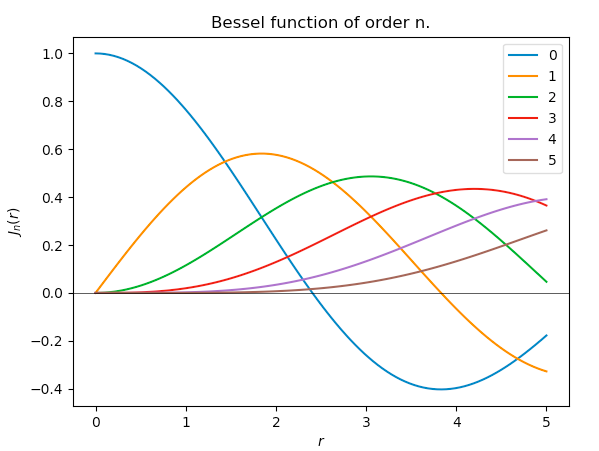
\includegraphics[width=8cm]{../figures/plot_bessel_int_order}
  \caption{Bessel functions of integer order.}\label{fig:bessel_int_problem}
\end{figure}

%------------------- neumann functions at the origin -----------------
\begin{propn}\label{propn:neumann_singular_at_origin}
  Neumann functions are singular at the origin.
\end{propn}
%
\begin{proof}
  From the definition of Neumann functions (definition \ref{defn:neumann_function}) we know that for $n$ integer
    \begin{equation}
      Y_n(z=0) = \lim_{\nu \rightarrow n} \frac{J_\nu(0) \cos (\nu \pi) - J_{-\nu}(0)}{\sin (\nu \pi)}
    \end{equation}
  %
  First, consider the limit of the numerator as $\nu \rightarrow$ integer. Then
  %
    \begin{gather*}
      J_\nu(0) \rightarrow
        J_n(0) = \left\{
          \begin{array}{c l}
               1 & n = 0 \\
               0 & n \neq 0
          \end{array}\right. \text{ from proposition \ref{propn:bessel_at_origin},}\\
      J_{-\nu}(0) \rightarrow
        (-1)^nJ_n(0) = (-1)^n\left\{
          \begin{array}{c l}
               1 & n = 0 \\
               0 & n \neq 0
          \end{array}\right.
          = \left\{
            \begin{array}{c l}
                 1 & n = 0 \\
                 0 & n \neq 0
            \end{array}\right. \text{ from proposition \ref{propn:bessel_int_order_identity}.}\\
      \text{Hence } J_{\pm\nu}(0) \rightarrow
        \left\{
          \begin{array}{c l}
               1 & n = 0 \\
               0 & n \neq 0
          \end{array}\right.
    \end{gather*}
  Additionally,
    \begin{gather*}
      \cos(\nu\pi) \rightarrow (-1)^n.
    \end{gather*}
  We broady have two cases for the numerator, $n=0$ and $n\neq 0$.
    \begin{gather*}
      J_\nu(0)\cos(\nu\pi) - J_\nu(0) \rightarrow
      \left\{
        \begin{array}{c l}
             1\times1-1=0 & n = 0 \\
             0\times1-0=0 & n \neq 0
        \end{array}\right.
    \end{gather*}
  Now for the denominator, clearly
    \begin{gather*}
      \sin(\nu\pi) \rightarrow 0.
    \end{gather*}
  This gives us the indeterminate limit $0/0$ at $x=0$ as $\nu \rightarrow$ integer.
\end{proof}
%
\begin{figure} \centering
  %
  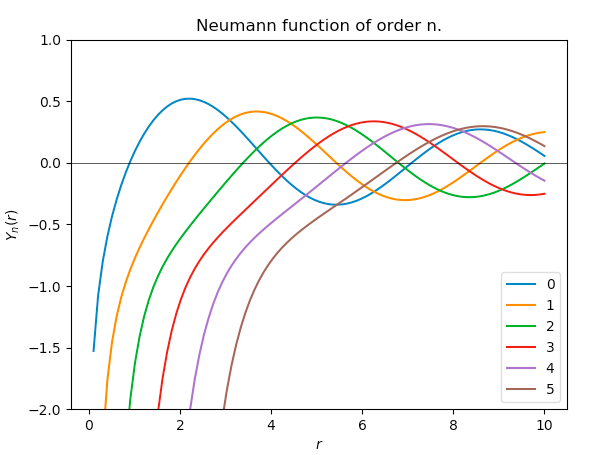
\includegraphics[width=8cm]{../figures/plot_neumann_int_order}
  \caption{Neumann functions of integer order.}\label{fig:neumann_int_problem}
  %
\end{figure}\par
%
\begin{propn}
  Hankel functions are singular at the origin.
\end{propn}
%
\begin{proof}
  This follows directly from the definition of Hankel functions for $n\in\bb{Z}$ (definition \ref{defn:hankel_func}), and can be proven in the same way as proposition \ref{propn:neumann_singular_at_origin}.
\end{proof}
%
\begin{figure} \centering
  %
  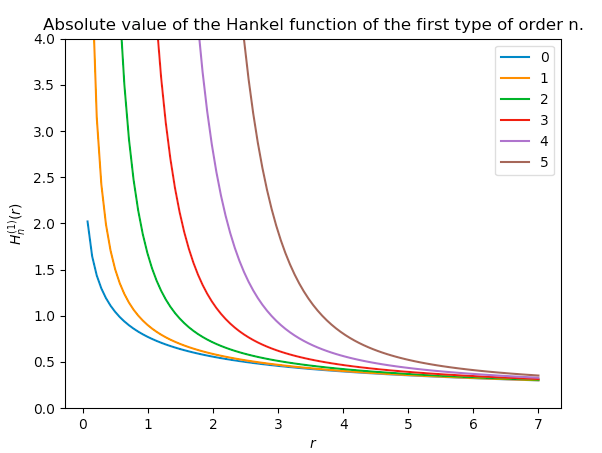
\includegraphics[width=8cm]{../figures/plot_hankel_int_order}
  \caption{Hankel functions of integer order.}\label{fig:hankel_int_problem}
  %
\end{figure}\par
